\section{Results}
\label{sec:-res}
In this section, we present both the results of our analysis on the 
data we have collected, and some preliminary connections between these 
results and the patterns identified in Section \ref{sec:-back}.


We measured the number of reblogs over all posts.  We found that the 
average post received approximately 30 reblogs.  However, the median 
number of reblogs over our study was 3.  This indicates that the 
distribution is highly skewed, with a great number of unpopular posts 
offset by a few massively reblogged posts.  In other words, the 
information displayed in Figure \cite{fig:-distance} showcases a 
sharp disparity that demarcates the line between regular posts, and 
posts that go viral: the difference between material from the typical 
user, and one who is, to use the topical colloquialism, 
``Tumblr famous.''  In Kwak et al.'s paper\cite{kwak2010twitter} on 
the mechanism of information spread through Twitter, they found that 
any tweet that was retweeted was likely to reach an average of 1,000 
users within a very small timing window.  As we do not have access to 
timing information at that level of granularity, we are unfortunately 
unable to make such classifications.


To place those numbers of reblogs in context, we have also measured 
the percentage of user posts that comprise content novel to the 
network, compared to posts that reblog existing content, distributing 
it further over the network.  In Figure \cite{fig:-deg}, we see that 
the average blog is composed of 70\% reblogged material, and that well 
over three quarters of the users surveyed reblog more content than they 
create.  



\begin{figure}[bht]
\centering
 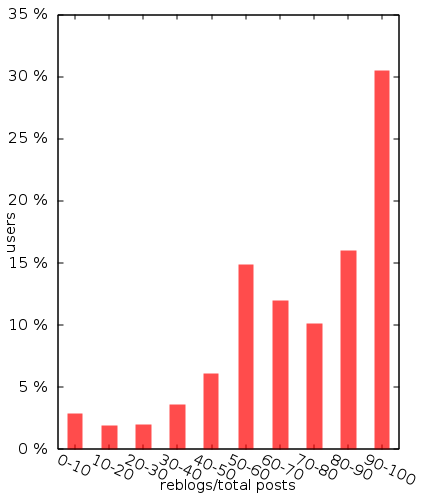
\includegraphics[width=3.5in]{degree}
  \caption{The bins on the X axis represent percentages of users, grouped by what percentage of their posts are reblogs.  The Y axis indicates the magnitude of the membership within this group.  Overall, we observe that blogs contain an average of 70\% reblogged material, and a median of 76\% reblogged material.}
  \label{fig:-deg}
\end{figure}

Figure \ref{fig:-deg} indicates that the majority of users spend more 
time reblogging others' content than adding their own to the network.


Figure \ref{fig:-pop} shows us that the most popular posts are text 
posts, followed most closely by image posts.  This suggests that Tumblr 
is not so far removed from classic blogging sites.


gifsets\cite{hillman2014tumblr}

\begin{figure}[bht]
\centering
 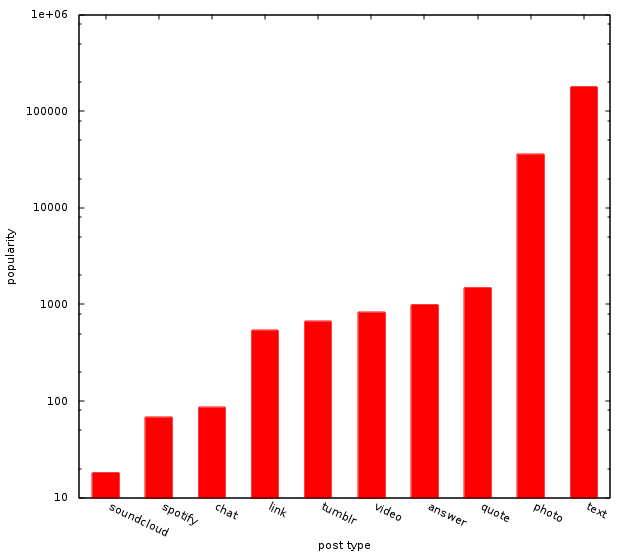
\includegraphics[width=3.5in]{popularity}
  \caption{The graph represents the note counts of all surveyed post types.  Note that the graph has a log scale on the y axis}
  \label{fig:-pop}
\end{figure}
This is particularly interesting in light of the 

%%% Local Variables: 
%%% mode: latex
%%% TeX-master: "main"
%%% End: 
